
\FloatBarrier
\section{Система Рёсслера} %  % {{{1 _ROSS_
\label{atu:sect:ross}

\LinkRef{
  ross: ASAU-14. ISDMCI-2011, ISDMCI-2012
  % ~/doc/tex/asau/asau14/atu/atu.tex
}

\subsection{Определение системы и анализ её динамики} %  % {{{2 _ross_task

In~\cite{neimark_stoch_chaos_vibro,koltsova_nl_dyn_chem,berje_order_in_chaos,chulichkcov_mm_ml_dyn}

\begin{equation}
\begin{cases}
  \dot{x}  = -y - z  ,  \\
  \dot{y}  = x + a y ,\\
  \dot{z}  = b + z \cdot ( x-c ) .
\end{cases}
\label{atu:eq:rossler}
\end{equation}

Здесь \(x\), \(y\), \(z\) -- переменные состояния системы,
которые соответствуют концентрациям основных реагентов
в моделируемой химической системе.
Соответственно \(a\), \(b\), \(c\) --
параметры, определяющие динамику системы
(в моделируемой системе определяются константами химического равновесия
и концентрациями вспомогательных реагентов).

При моделировании данной системы положим
\(a=0.25\), \(b=1\).
В этом случае параметр \(c\) определяет
тип динамики системы.
Определение значения данного параметра и будет
целью задачи идентификации.

В данной системе нет внешнего входного сигнала \( u(t) \).
Это объясняется тем, что за счет
поддержания постоянных концентраций вспомогательных
компонент, постоянного пополнения исходных веществ
и удаления продуктов реакции система обладает
собственным источником энергии, который обеспечивает
динамику системы и при отсутствии
внешнего воздействия.

Как и другие системы хаотической динамики, система Ресслера
не позволяет построить систему идентификации, основанную
на формировании критерия качества идентификации
как меры близости непосредственных значений выходных сигналов
объекта \( x_0(t) \) и модели \( x_m(t) \).
Более того, сам вид поведения данной системы может значительно изменяться
при малых изменениях параметров, совершая переход от
хаотического к сложно-периодическому и обратно.

При малых значениях параметра (\(c \approx 3 \))
система проявляет регулярную динамику,
совершая колебательное движение вокруг точки
неустойчивого равновесия~(рис.~\ref{atu:f:ross_attractor_0300}).

\begin{figure}[ht!]
\begin{center}
  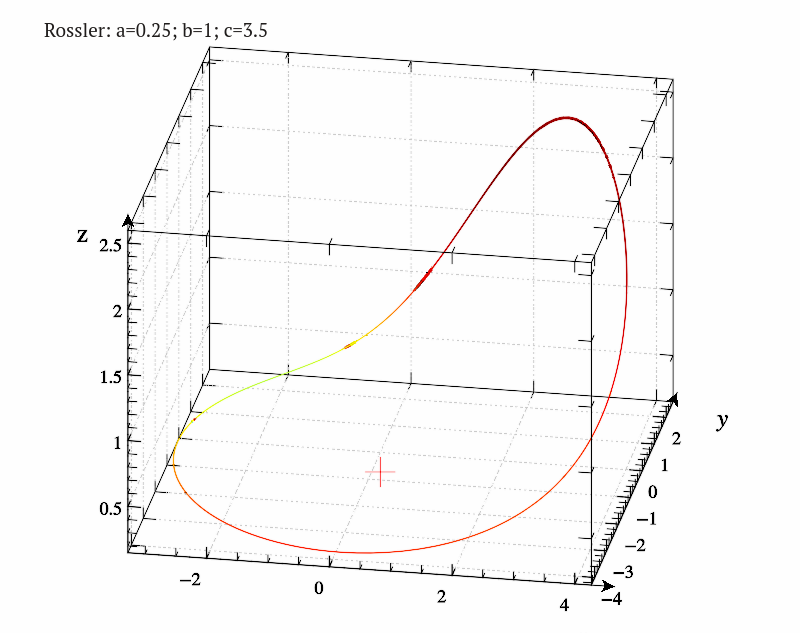
\includegraphics[width=0.49\textwidth]{p/cha/ross/ross0-p_xyz_c=03x50.png}
  \hfill
  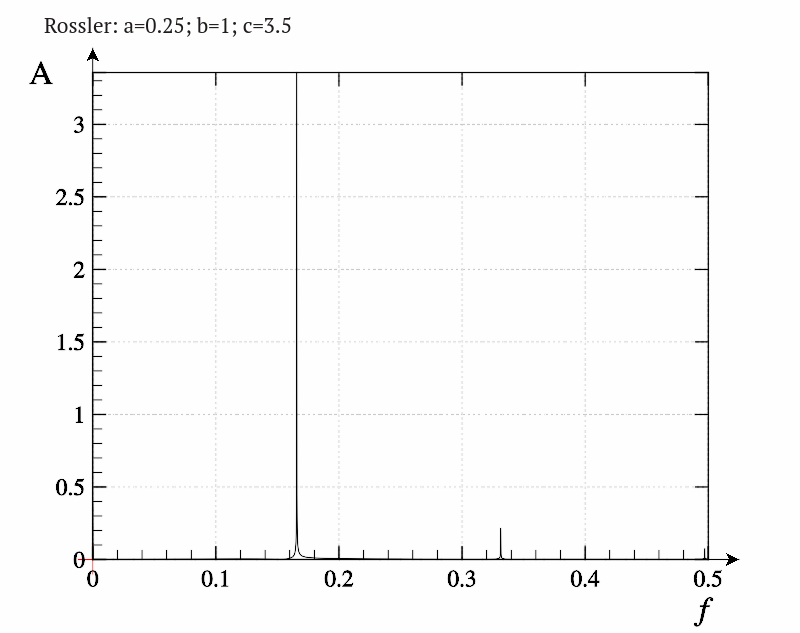
\includegraphics[width=0.49\textwidth]{p/cha/ross/ross_f-p_f_c=03x50.png}
\end{center}
  \caption{Аттрактор и спектр системы Рёсслера (\ref{atu:eq:rossler}) в режиме регулярных колебаний ($c=3.5$)}
\label{atu:f:ross_attractor_0300}
\end{figure}

При увеличении значения параметра \(c\) происходит удвоение периода,
поведение системы становится все более сложным, и в определенном
диапазоне значений параметра система демонстрирует
хаотическую динамику(рис.~\ref{atu:f:ross_attractor_0588}).

\begin{figure}[ht!]
\begin{center}
  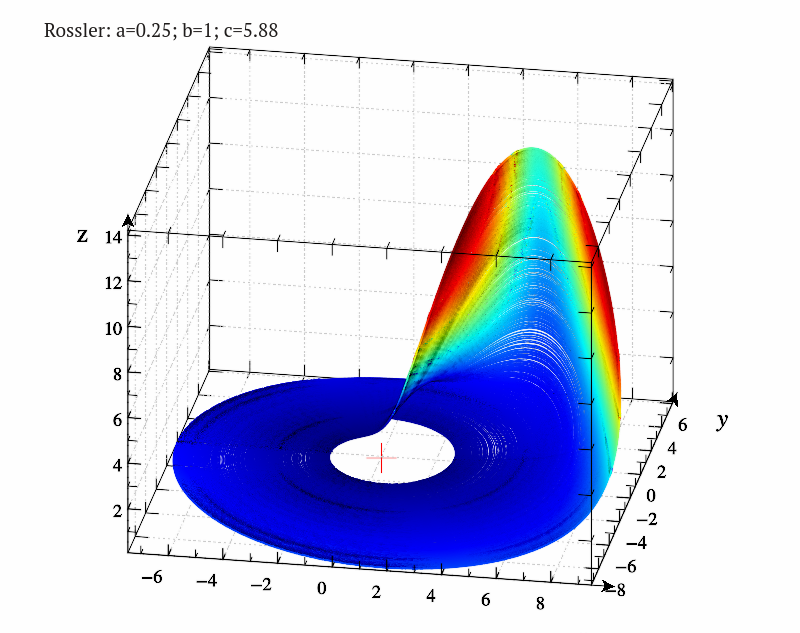
\includegraphics[width=0.49\textwidth]{p/cha/ross/ross0-p_xyz_c=05x88.png}
  \hfill
  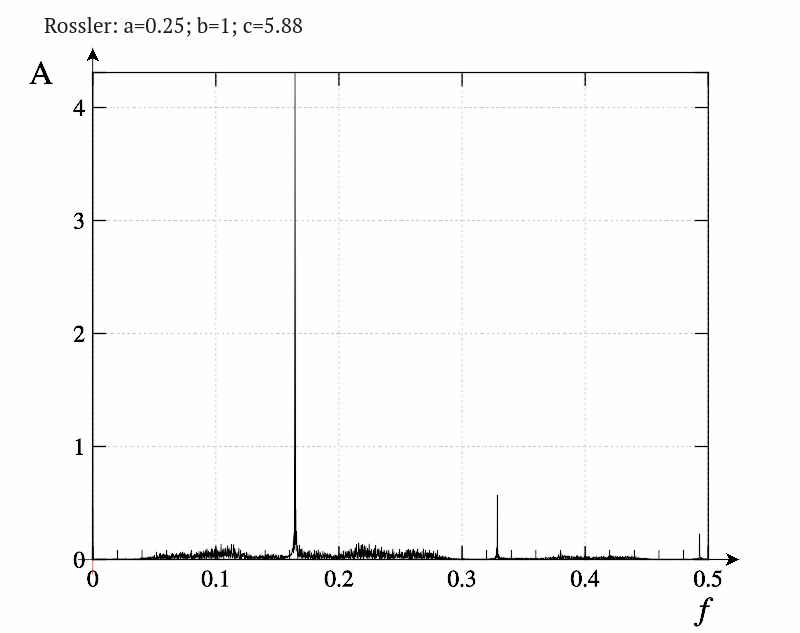
\includegraphics[width=0.49\textwidth]{p/cha/ross/ross_f-p_f_c=05x88.png}
\end{center}
  \caption{Аттрактор и спектр системы Рёсслера (\ref{atu:eq:rossler}) в режиме хаотических колебаний ($c=5.88$)}
\label{atu:f:ross_attractor_0588}
\end{figure}

Прослеживается отличие спектра системы Рёсслера в хаотическом режиме
от аналогичных условий для систем Лоренца. Отличие заключается в том, что
существует ярко выраженный пик, соответствующий базовой частоте,
а области сплошного спектра характеризуются небольшой амплитудой.
При некоторых больших значениях параметра $c$
область сплошного спектра становится более заметной,
однако общая структура спектра остаётся такой же.


При дальнейшем увеличении значения параметра \(c\)
наблюдаются переходы от хаотического к сложно-периодическому
(рис.~\ref{atu:f:ross_attractor_2500})
и  обратно.

\begin{figure}[ht!]
\begin{center}
  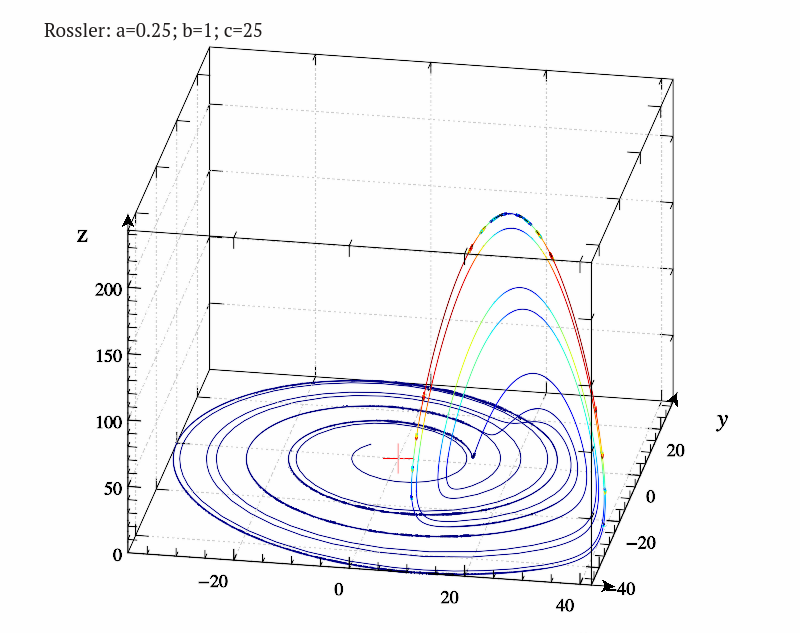
\includegraphics[width=0.49\textwidth]{p/cha/ross/ross0-p_xyz_c=25x00.png}
  \hfill
  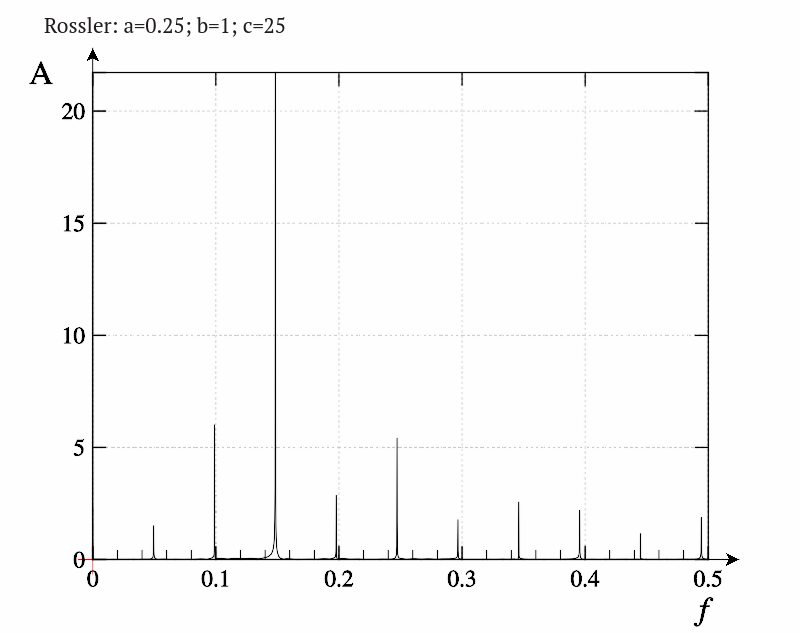
\includegraphics[width=0.49\textwidth]{p/cha/ross/ross_f-p_f_c=25x00.png}
\end{center}
  \caption{Аттрактор и спектр системы Рёсслера (\ref{atu:eq:rossler}) в режиме сложно-периодических колебаний ($c=25.0$)}
\label{atu:f:ross_attractor_2500}
\end{figure}

При этом наблюдается линейчатый спектр. Также при
таких периодах может скачкообразно изменятся
размер области, в которую вписан аттрактор.
В этом смысле система Рёсслера потенциально является более сложной
для идентификации, чем системы Лоренца и ``Sprott A''.

% Идентифицируемый параметр:
% $ c \in [2; 50] $, $c_0=5.88$.
%
% Остальные параметры:
% \( a \in (0, 0.35 ) \), $a_0=0.25$,
% \(b \in[0;4] \), $b_0=1$.


% }}}2

\subsection{Анализ и выбор критериев}  % {{{2

Критерий
$ z_{\max}$, $ \overline{z} $.

\begin{figure}[ht!]
\begin{center}
  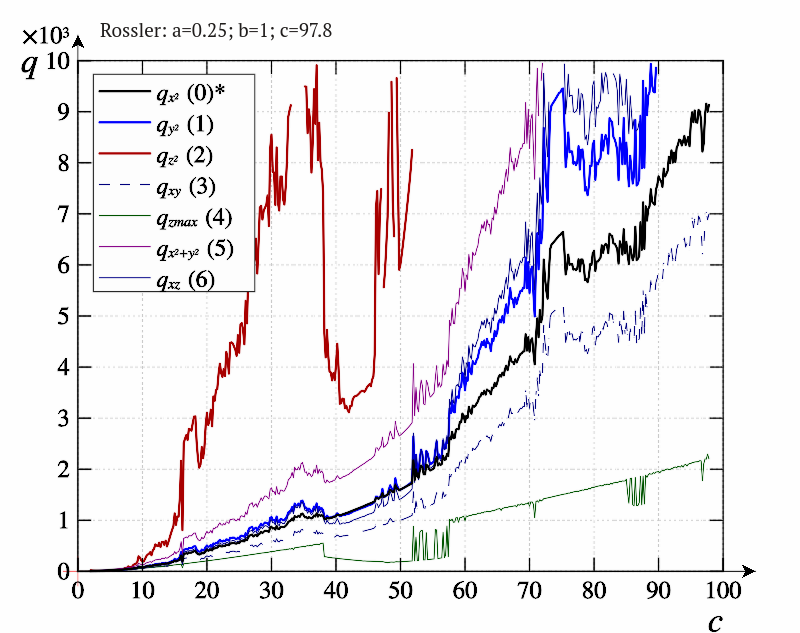
\includegraphics[width=0.49\textwidth]{p/cha/ross/ross_q-p_q.png}
  \hfill
  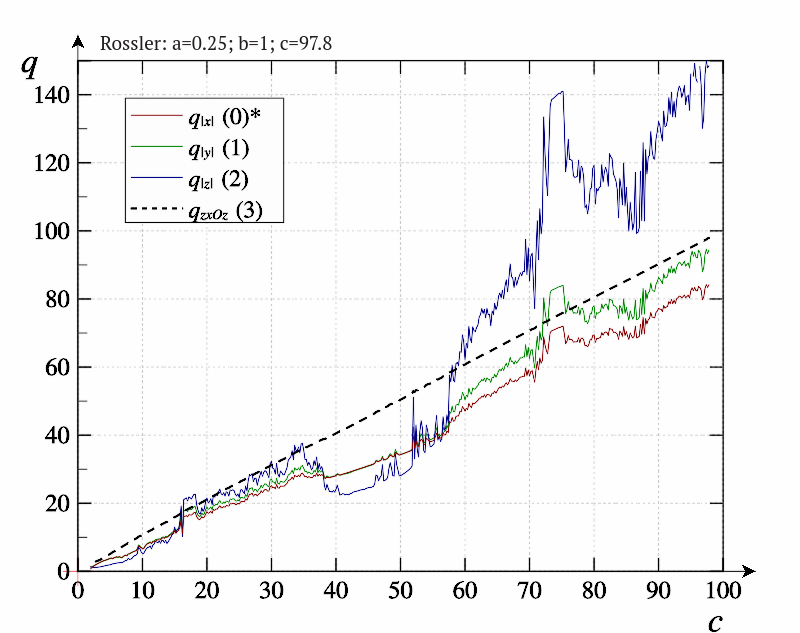
\includegraphics[width=0.49\textwidth]{p/cha/ross/ross_q-p_q1.png}
\end{center}
  \caption{Рассматриваемые критерии для системы Рёсслера}
\label{atu:f:ross_q}
\end{figure}

\begin{figure}[ht!]
\begin{center}
  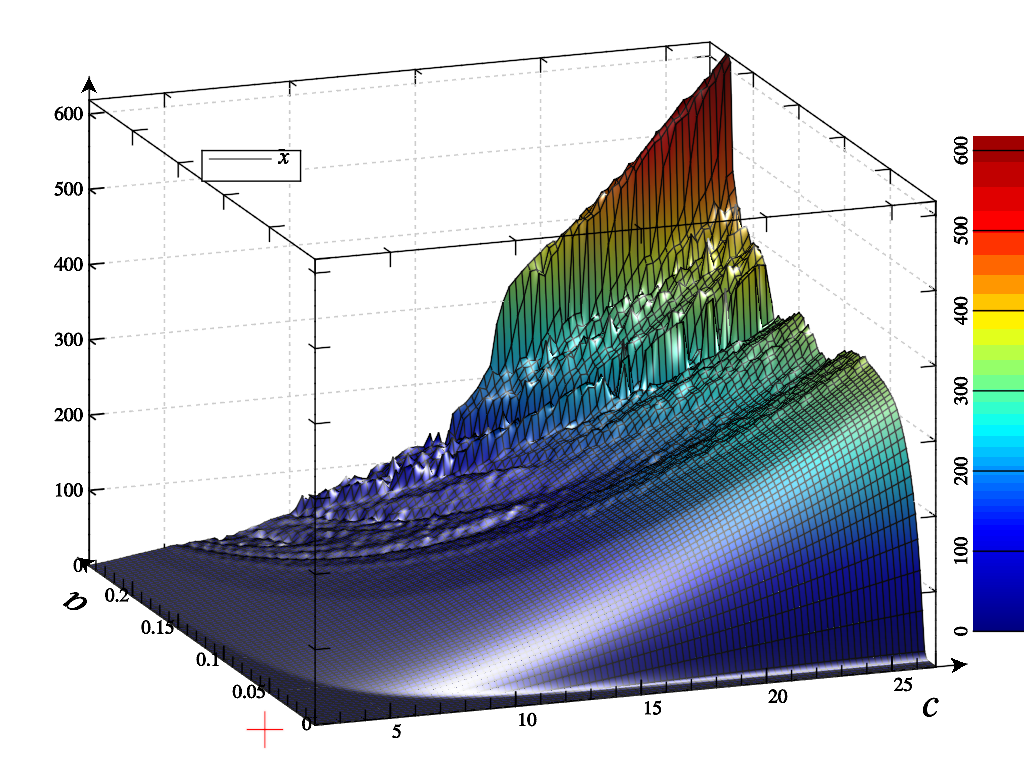
\includegraphics[width=0.49\textwidth]{p/cha/ross/ross_pwr-x_a_c.png}
  \hfill
  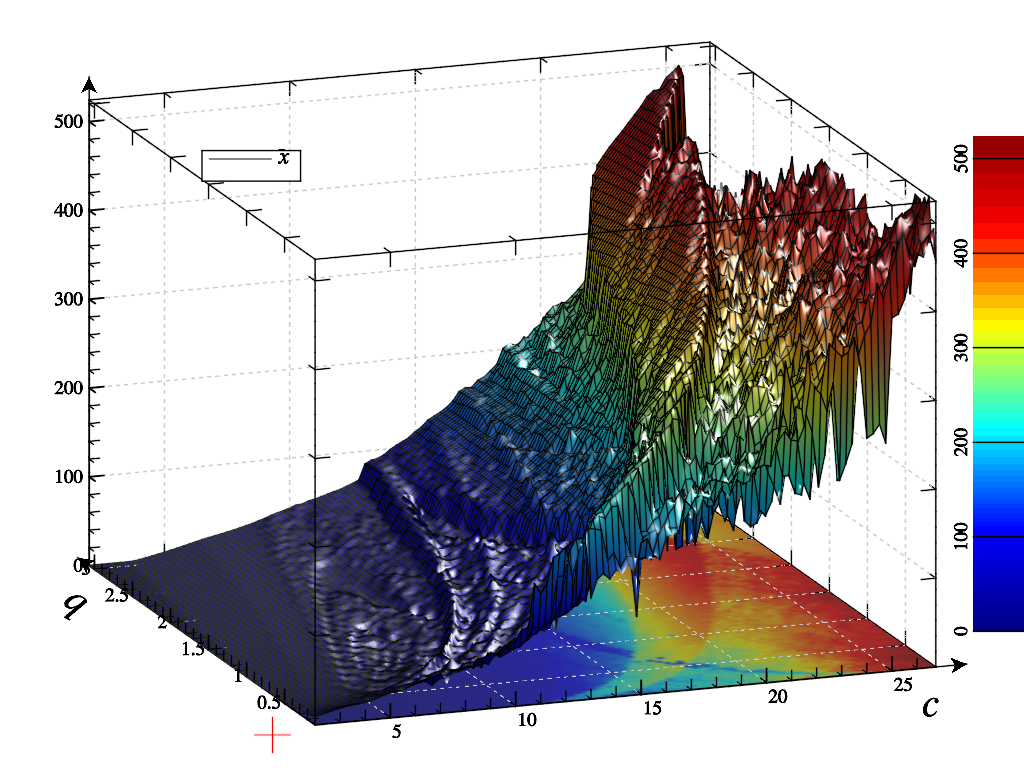
\includegraphics[width=0.49\textwidth]{p/cha/ross/ross_pwr-x_b_c.png}
\end{center}
  \caption{Зависимости $q_{x^2}(a,c)$ и  $q_{x^2}(b,c) $ для системы Рёсслера}
\label{atu:f:ross_q_x2_ac_bc}
\end{figure}

\begin{figure}[ht!]
\begin{center}
  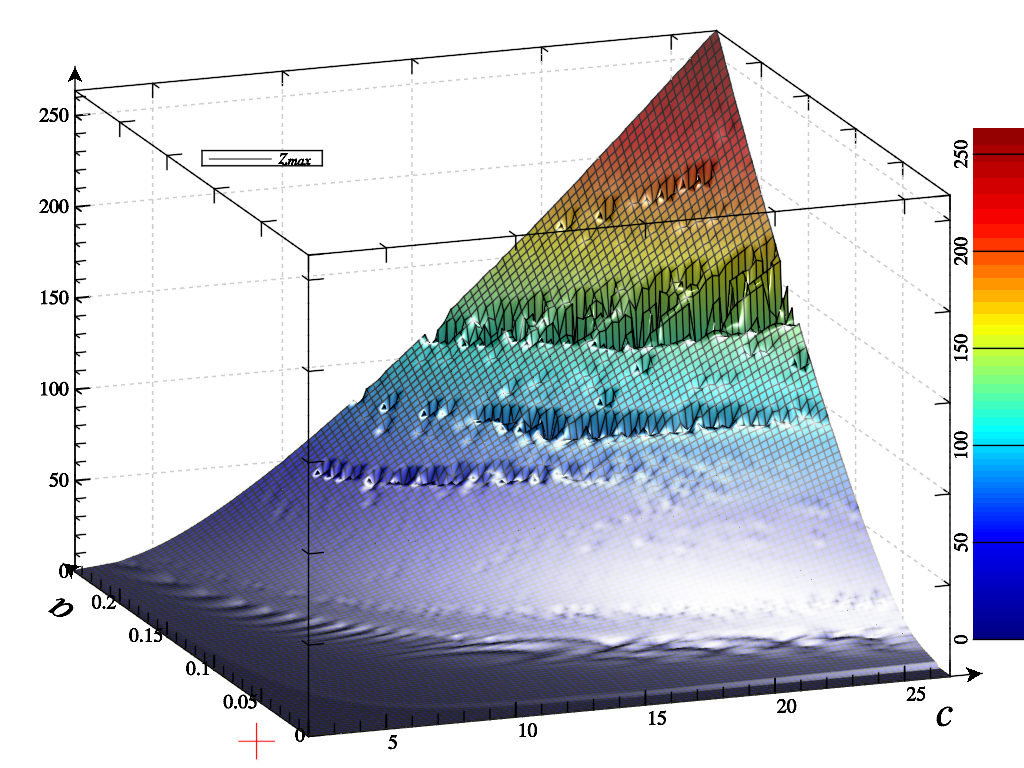
\includegraphics[width=0.49\textwidth]{p/cha/ross/ross_zmax_a_c.png}
  \hfill
  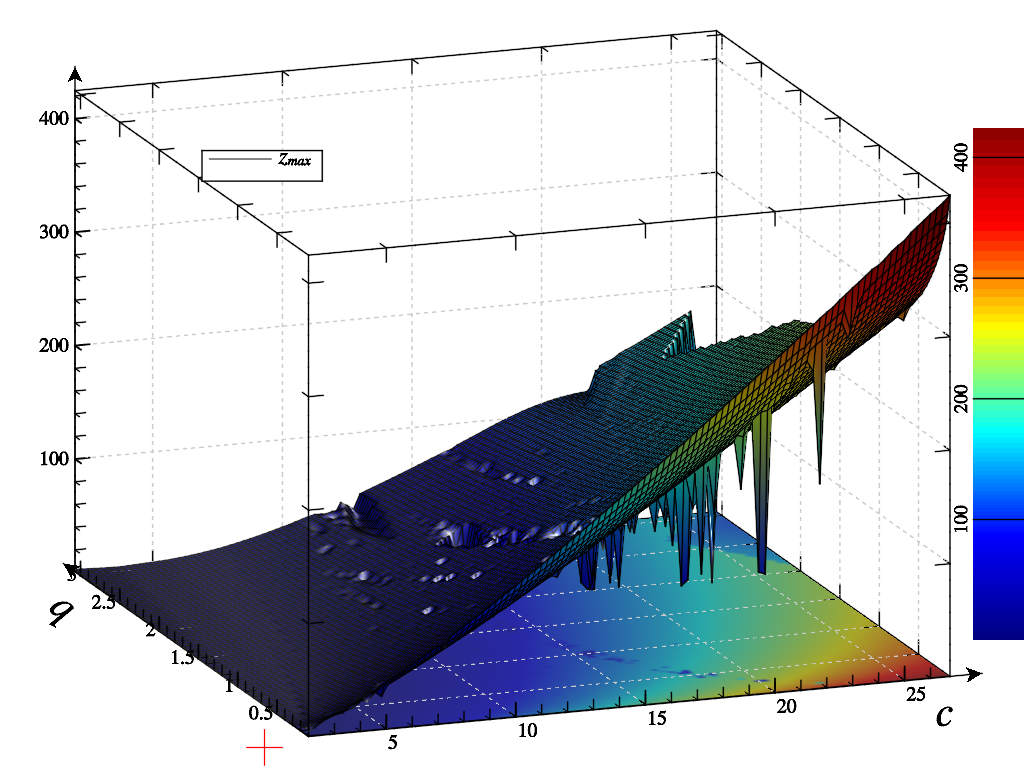
\includegraphics[width=0.49\textwidth]{p/cha/ross/ross_zmax_b_c.png}
\end{center}
  \caption{Зависимости $q_{zmax}(a,c)$ и  $q_{zmax}(b,c) $ для системы Рёсслера}
\label{atu:f:ross_q_zmax_ac_bc}
\end{figure}



% }}}2

\subsection{Тестовая задача идентификации для системы Рёсслера}  % {{{2


% }}}2

\subsection{Влияние параметров системы идентификации на ошибку идентификации для системы Рёсслера}  % {{{2

% }}}2

\subsection{Зависимости значений критериев идентификации при изменении двух параметров системы Рёсслера}  % {{{2

% }}}2



\subsection{Выводы}  % {{{2

Выводы

% }}}2


% }}}1

% vim: fdm=marker foldlevelstart=3 fdc=4 ft=tex
